\documentclass[10pt,a4paper]{article}
%% Language and font encodings
\usepackage[british]{babel}
\usepackage[utf8]{inputenc}
\usepackage[T1]{fontenc}
%% Sets page size and margins
\usepackage[a4paper,top=2cm,bottom=2cm,left=2.5cm,right=2.5cm,marginparwidth=1.5cm]{geometry}
%% Useful packages
\usepackage{amsmath}
\usepackage{graphicx}
\usepackage[colorinlistoftodos]{todonotes}
\usepackage[colorlinks=true, allcolors=blue,]{hyperref}
\usepackage{authblk}
\usepackage[backend=biber,style=numeric-comp]{biblatex}
\usepackage{listings}
\usepackage{xcolor}
\usepackage{amsmath} \allowdisplaybreaks% lets align equations break over pages.
\usepackage{amssymb}
\usepackage{caption}
\usepackage{svg}
\usepackage{cleveref}
\definecolor{codegreen}{rgb}{0,0.6,0}
\definecolor{codegray}{rgb}{0.5,0.5,0.5}
\definecolor{codepurple}{rgb}{0.58,0,0.82}
\definecolor{backcolour}{rgb}{0.95,0.95,0.92}


% \addbibresource{references.bib}

\lstdefinestyle{mystyle}{
  backgroundcolor=\color{backcolour},
    commentstyle=\color{codegreen},
    keywordstyle=\color{magenta},
    numberstyle=\tiny\color{codegray},
    stringstyle=\color{codepurple},
    basicstyle=\ttfamily\footnotesize,
    breakatwhitespace=false,
    breaklines=true,
    captionpos=b,
    keepspaces=true,
    numbers=left,
    numbersep=5pt,
    showspaces=false,
    showstringspaces=false,
    showtabs=false,
    tabsize=2
}
\lstset{style=mystyle}

\graphicspath{{./img/}}

%% Title
\title{
  {\Huge Simulation and Performance Evaluation}\\
  \huge Homework 4\\
}

\author{Blascovich Alessio and Di Noia Matteo}

\begin{document}

\maketitle

\section*{Simulation Set-Up}

In the simulation the times, between two consecutive packet arrivals and the service time for a packet, follow an exponential distribution of parameters \(\lambda\) and \(\mu\) respectively.

The simulation consists in a FIFO queue of packets arrived that need to be served by a processor.

%TODO explain the computation of the variance and state the confidence interval level used
For measuring it we computed the mean estimators of the parameters searched and also their variance which was used to compute a confidence interval (CI) with 95\% confidence level.

\section*{Exercise 1}

We can start by showing how a simulation evolves over time with particular focus on the number of packets in the queue and in processing. Assuming a single packet can be processed at a time.

\begin{center}
  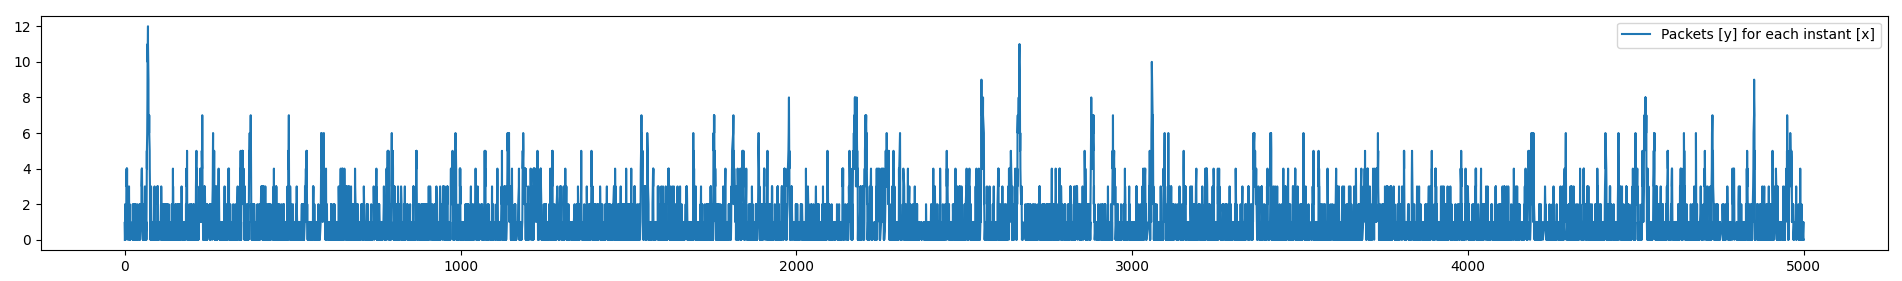
\includegraphics[width=\textwidth]{whole-simulation.png}
  \captionof{figure}{Number of packets in the queue throughout a simulation with \(\lambda = 1\) and \(\mu = 2\)}
\end{center}

% TODO put exponential and log graph about the quantity of packets over time
We started y executing the simulation and plotting the distribution of time in which the simulation had a number of packet, given by summing the queues elements plus the packet that is being processed, if present. By doing so we found out as expected that such distribution is also an exponential. We can be sure of this by plotting with logarithm scale, compute the line that best fit the new data and compute the fit of such a line. The resulting line is in the case of image \ref{} is \(-0.385 \cdot x +  9.710\). This line is a good fit for our distribution as the \(R^2\) test of fitness of a line return a value of 0.992 (where 1 is a perfect fit).
From this we could easily construct, by elevating to the power of \(e\) the line function, the best fit exponential.
\begin{center}
	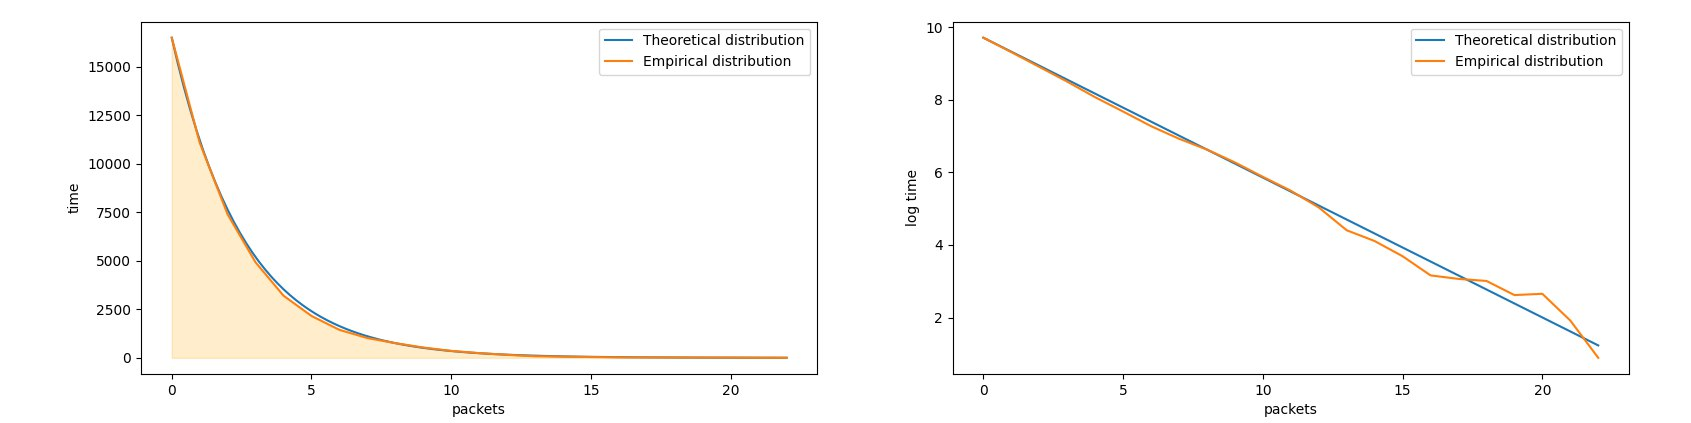
\includegraphics[width=\textwidth]{img/time-with-fixed-packet-n.png}
	\captionof{figure}{Total length of time in which \(x\) packets are in queue or in processing with \(\lambda = 1\) and \(\mu = 1.5\)}
	\label{fig:time-with-fixed-packet-n}
\end{center}


\subsection*{Independent Replication}

We started using ``Independent Replication'' as method to gather information about the number of packets in the queue given a time instant. This method has many advantages, especially for finite state simulations, but can be used as well for steady state analysis; although you have to take into consideration some possible issues such as initialization problem, introducing periodicity and some others. As such we used this method for qualitative analysis and to compare the other methods used.

\begin{center}
	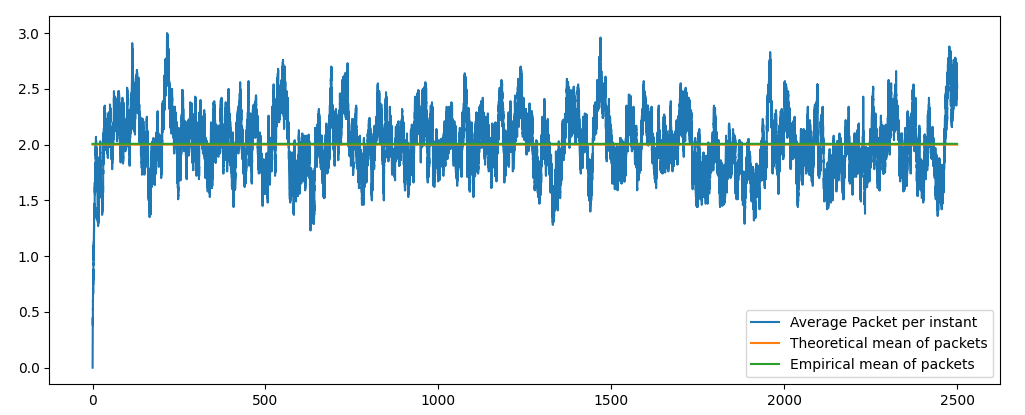
\includegraphics[width=0.7\textwidth]{independent-replication-with-bias.png}
	\captionof{figure}{Independent replication with initialization bias, \(\lambda = 1\) and \(\mu = 1.5\)}
	\label{fig:independent-replication-with-bias}
\end{center}

We started using ``Independent Replication'' as method to gather information about the number of packets in the queue given a time instant. This method has many advantages, especially for finite state simulations, but can be used as well for steady state analysis; although you have to take into consideration some possible issues such as initialization problem, introducing periodicity and some others. As such we used this method for qualitative analysis and to compare the other methods used.


Using ``Independent Replication'' we had to take into consideration the initialization bias that is clearly visible in the left hand-side of~\Cref{fig:independent-replication-with-bias}. This bias is caused by all simulations starting with an empty queue, i.e. 0 packets, at the same time namely instant 0. To overcome this problem there are many solutions:
\begin{itemize}
\item Starting the simulation at a different initial time, starting gathering data after all the simulation have started;
\item Running the simulation for a longer period of time;
\item Discard the first data, using some criteria.
\end{itemize}

We chose the latter method by discarding the first \emph{n} time instants from each simulation, with \emph{n} defined as a multiple of the average number of packets in the system in stationary conditions. However this technique works only in non-divergent simulations (\(\lambda\geq\mu\)) as in those cases the average tends to infinite, this is the case for all the other methods that use the average number of packets in the system. In those cases it is possible to only compute a function describing the climb rate of the average number of packets.

\begin{center}
  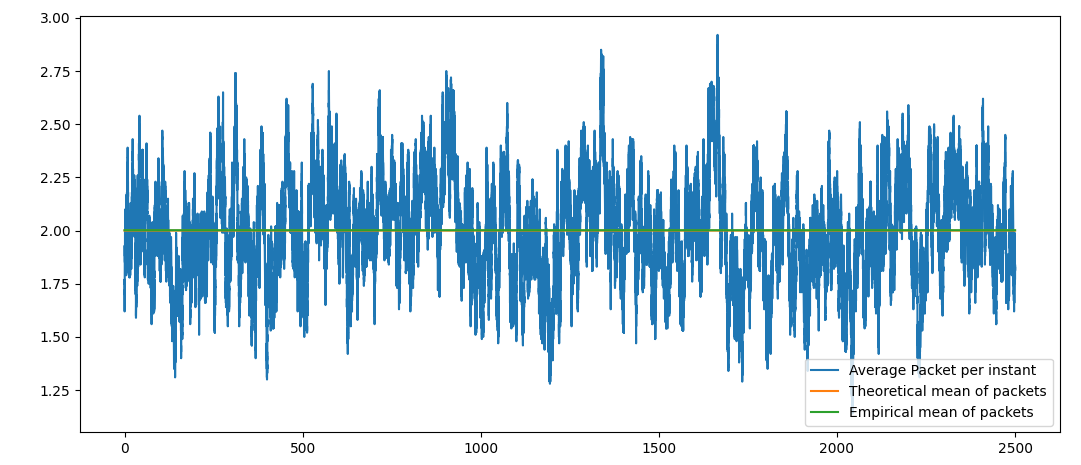
\includegraphics[width=0.7\textwidth]{independent-replication-without-bias.png}
  \captionof{figure}{Independent replication without initialization bias, \(\lambda = 1\) and \(\mu = 1.5\)}
  \label{fig:independent-replication-without-bias}
\end{center}

Discarding the first \emph{n} time instant we passed from an average of \(2.007 \pm 0.0438\)(\Cref{fig:independent-replication-with-bias}) to an average of \(2.002 \pm 0.0405\)(\Cref{fig:independent-replication-without-bias}), with a theoretical value of 2. While the graph in~\Cref{fig:independent-replication-without-bias} is more representative of the real average over time of a stationary conditions, the obtained average and relative CI do not get much better since the length of the simulation, already partially overwhelm the initialization bias.

\subsection*{Overlapping Batch Means}

Then we used ``Overlapping Batch Means'' as method to estimate data mean and variance. Since for this method only one simulation is involved, we decided to augment the length of it. The new length used was \(\mathit{number~of~simulations}\times\mathit{length~of~single~simulation}\) used for the ``Independent Replication'' method.

To use this method we must have:
\begin{itemize}
\item Normally distributed batch data;
\item IID data.
\end{itemize}

The second condition is easily verified since every time interval is generated independently and with the same parameters. For the former condition is verified if the batch is large enough. To satisfy both conditions we picked as batch size \(\mathit{simulation~length} / 1000\) and as number of batch \(10000\) so that they are also overlapping for sure.

Given the theoretical mean is still 2, since we used the same parameters. Some of the empirical means obtained are \( 1.987 \pm 0.0058\), \(2.006 \pm 0.0059\), \(2.010 \pm 0.0062\) and \(1.997 \pm 0.0058\). The CIs obtained are strongly under-estimate for the confidence level of 95\%, to reach the confidence level the obtained CIs should be doubled in size. This problem is due to the fact that this method tends to under-estimate the variance and the fact that probably we are not completely fulfilling the prerequisites of this method.

To conclude, we expected to achieve better results using this method; however the ``Independent Replication'' method gave better results (especially confidence intervals) and was easier to work with.

\subsection*{Varying parameters}

%TODO Quote the usage of rho insert bottom left ex1 graph with rho = 2, 1, 0.90, 0.1
We then analyzed the convergence of the system with different parameters \(\lambda\) and \(\mu\). To be exact we analyzed the system behavior for different value of \(\rho\) which is defined as the rate \(\frac \lambda \mu\). We expect value of \(\rho \ge 1\) to diverge, value closer to 1 to take accumulate larger queue with higher probability while value closer to 0 to tend to be have smaller queue and dispatch them quickly.

% TODO 4 images (make a grid 2x2)

\begin{figure}[ht!]
	\centering
	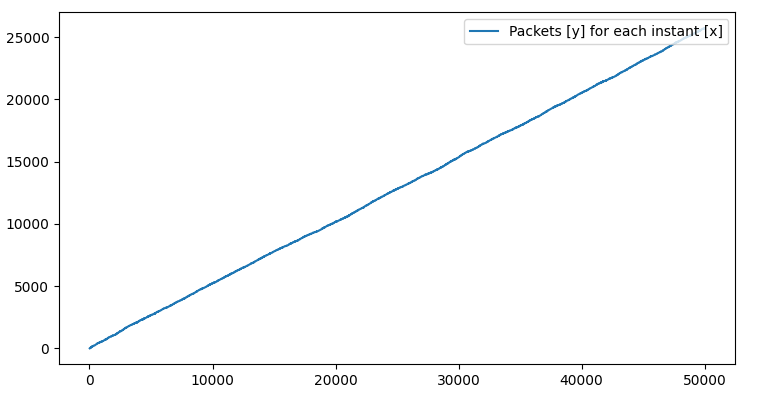
\includegraphics[width=0.45\linewidth]{img/pho2}
	\label{fig:pho2}
	~
	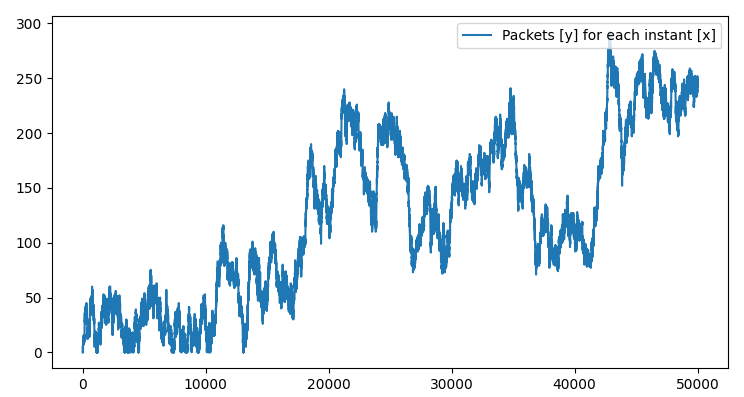
\includegraphics[width=0.45\linewidth]{img/rho1}
	\label{fig:rho1}

	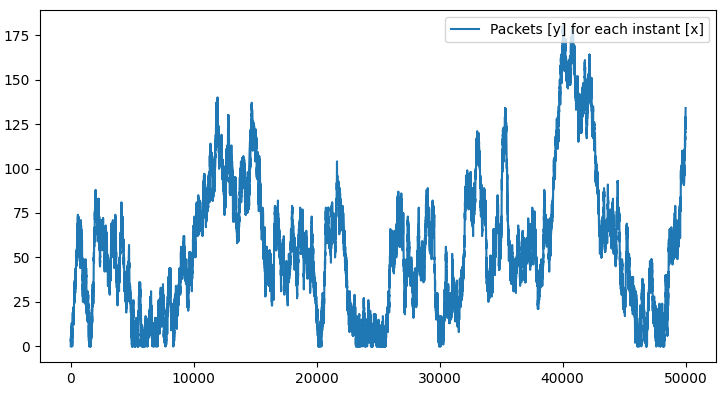
\includegraphics[width=0.45\linewidth]{img/rho0.99}
	\label{fig:rho099}
	~
	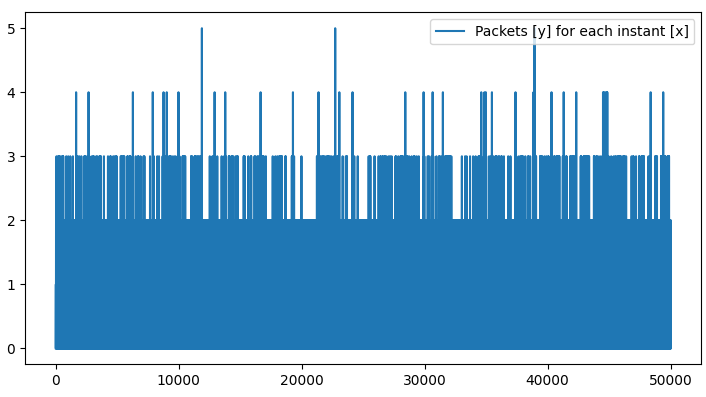
\includegraphics[width=0.45\linewidth]{img/rho0.1}
	\label{fig:rho010}

	\caption{TODO} % TODO
	\label{img:data-vis}
\end{figure}


As it is possible to see in the two rows: \ref{} and \ref, the value follow what we expected. In the first ones, the two graph show two simulation with  \(\rho \ge 1\), and as such diverging. The difference between the two is that while the first having a much more rapid rate of climb, almost constant; the other climb much slower. On the second row instead we see two cases with \(\rho \le 1\), in this case we see that the first example almost resemble the divergent case, creating large queue; instead the second has a much smaller \(\rho\) and as such most of packets are quickly dispatched and because of this the queue very often empty with at most a packet currently being processed.



\section*{Exercise 2}

% TODO quote method chosen, pseudo-codes, naïf values and refined values, and observation about data semantics and non-naïf is better
% TODO Intro
% TODO Image
To compute the variance of the mean two methods where employed: the naive method, which is the variance of all the measurements and the post-stratification, defining the stratum as the number of packet in queue in the system when the packet arrive.
% TODO Pseudo code
The results of this two methods when ...


\end{document}
